
%%%%%%%% ICML 2018 EXAMPLE LATEX SUBMISSION FILE %%%%%%%%%%%%%%%%%

\documentclass{article}

% Recommended, but optional, packages for figures and better typesetting:
\usepackage{microtype}
\usepackage{graphicx}
\usepackage{subfigure}
\usepackage{booktabs} % for professional tables

% hyperref makes hyperlinks in the resulting PDF.
% If your build breaks (sometimes temporarily if a hyperlink spans a page)
% please comment out the following usepackage line and replace
% \usepackage{icml2018} with \usepackage[nohyperref]{icml2018} above.
\usepackage{hyperref}

% Attempt to make hyperref and algorithmic work together better:
\newcommand{\theHalgorithm}{\arabic{algorithm}}

\newcommand{\system}{EC2.0~}

% Use the following line for the initial blind version submitted for review:
\usepackage{icml2018}


\usepackage{hyperref}       % hyperlinks
\usepackage{url}            % simple URL typesetting
\usepackage{booktabs}       % professional-quality tables
\usepackage{amsfonts}       % blackboard math symbols
\usepackage{nicefrac}       % compact symbols for 1/2, etc.
\usepackage{microtype}      % microtypography

\usepackage{listings}
\usepackage{amsthm}
% use Times
\usepackage{times}
% For figures
\usepackage{graphicx} % more modern
%\usepackage{epsfig} % less modern
\usepackage{subfig} 
\usepackage{fancyvrb}


\usepackage{caption}
\usepackage{subcaption}

\fvset{fontsize=\footnotesize}

\usepackage{amssymb}
\usepackage{listings}
\usepackage{wrapfig}
\usepackage{tabularx}


\usepackage{verbatim}
 \usepackage{booktabs}
 % For algorithms
\usepackage{algorithm}
\usepackage{algorithmic}
\usepackage{tikz}
\usetikzlibrary{fit,bayesnet}
%\usetikzlibrary{arrows.meta}
\usetikzlibrary{positioning}
%\usetikzlibrary{decorations.text,decorations.pathreplacing}
%\usetikzlibrary{decorations.pathmorphing}
\usepackage{dsfont}
\usepackage{amsmath}
\usepackage{hyperref}
\DeclareMathOperator*{\argmin}{arg\,min} % thin space, limits underneath in displays
\DeclareMathOperator*{\argmax}{arg\,max} % thin space, limits underneath in displays
\DeclareMathOperator{\argmin}{argmin} % no space, limits underneath in displays



% Packages hyperref and algorithmic misbehave sometimes.  We can fix
% this with the following command.

\newcommand{\Expect}{\mathds{E}} %{{\rm I\kern-.3em E}}
\newcommand{\indicator}{\mathds{1}} %{{\rm I\kern-.3em E}}
\newcommand{\expect}{\mathds{E}} %{{\rm I\kern-.3em E}}
\newcommand{\probability}{\mathds{P}} %{{\rm I\kern-.3em P}}



% If accepted, instead use the following line for the camera-ready submission:
%\usepackage[accepted]{icml2018}

% The \icmltitle you define below is probably too long as a header.
% Therefore, a short form for the running title is supplied here:
\icmltitlerunning{Inducing Domain Specific Languages for Bayesian Program Learning}

\begin{document}

\twocolumn[
\icmltitle{Inducing Domain Specific Languages for Bayesian Program Learning}

% It is OKAY to include author information, even for blind
% submissions: the style file will automatically remove it for you
% unless you've provided the [accepted] option to the icml2018
% package.

% List of affiliations: The first argument should be a (short)
% identifier you will use later to specify author affiliations
% Academic affiliations should list Department, University, City, Region, Country
% Industry affiliations should list Company, City, Region, Country

% You can specify symbols, otherwise they are numbered in order.
% Ideally, you should not use this facility. Affiliations will be numbered
% in order of appearance and this is the preferred way.
\icmlsetsymbol{equal}{*}

\begin{icmlauthorlist}
\icmlauthor{Aeiau Zzzz}{equal,to}
\icmlauthor{Bauiu C.~Yyyy}{equal,to,goo}
\icmlauthor{Cieua Vvvvv}{goo}
\icmlauthor{Iaesut Saoeu}{ed}
\icmlauthor{Fiuea Rrrr}{to}
\icmlauthor{Tateu H.~Yasehe}{ed,to,goo}
\icmlauthor{Aaoeu Iasoh}{goo}
\icmlauthor{Buiui Eueu}{ed}
\icmlauthor{Aeuia Zzzz}{ed}
\icmlauthor{Bieea C.~Yyyy}{to,goo}
\icmlauthor{Teoau Xxxx}{ed}
\icmlauthor{Eee Pppp}{ed}
\end{icmlauthorlist}

\icmlaffiliation{to}{Department of Computation, University of Torontoland, Torontoland, Canada}
\icmlaffiliation{goo}{Googol ShallowMind, New London, Michigan, USA}
\icmlaffiliation{ed}{School of Computation, University of Edenborrow, Edenborrow, United Kingdom}

\icmlcorrespondingauthor{Cieua Vvvvv}{c.vvvvv@googol.com}
\icmlcorrespondingauthor{Eee Pppp}{ep@eden.co.uk}

% You may provide any keywords that you
% find helpful for describing your paper; these are used to populate
% the "keywords" metadata in the PDF but will not be shown in the document
\icmlkeywords{Machine Learning, ICML}

\vskip 0.3in
]

% this must go after the closing bracket ] following \twocolumn[ ...

% This command actually creates the footnote in the first column
% listing the affiliations and the copyright notice.
% The command takes one argument, which is text to display at the start of the footnote.
% The \icmlEqualContribution command is standard text for equal contribution.
% Remove it (just {}) if you do not need this facility.

%\printAffiliationsAndNotice{}  % leave blank if no need to mention equal contribution
\printAffiliationsAndNotice{\icmlEqualContribution} % otherwise use the standard text.

\begin{abstract}
This document provides a basic paper template and submission guidelines.
Abstracts must be a single paragraph, ideally between 4--6 sentences long.
Gross violations will trigger corrections at the camera-ready phase.
\end{abstract}

\section{Introduction}

Imagine an agent faced with a suite of new problems totally different
from anything it has seen before. It has at its disposal a basic set
of primitive actions it can compose to build solutions to these problems, but
it is no idea what kinds of primitives are appropriate for which
problems nor does it know the higher-level vocabulary in
which solutions are best expressed.
How can our agent get off the ground?

The AI and machine learning literature contains two broad takes on this problem.
The first take is that the agent should come up with a better representation of the space of solutions,
for example, by inventing new primitive actions: see \emph{options} in reinforcement learning~\cite{stolle2002learning}, the EC algorithm in program synthesis~\cite{Dechter:2013:BLV:2540128.2540316}, or predicate invention in inductive logic programming~\cite{muggleton2015meta}.
The second take is that the agent should learn a discriminative model mapping problems to a distribution over solutions: for example, policy gradient methods in reinforcement learning or neural models of program synthesis~\cite{devlin2017robustfill,balog2016deepcoder}.
Our contribution is a general algorithm for fusing these two takes on the problem:
we propose jointly inducing a representation language, called a \emph{Domain Specific Language} (DSL),
alongside a bottom-up discriminative model that regresses from problems to solutions.
We evaluate our algorithm on four domains:
building Boolean circuits; symbolic regression; FlashFill-style~\cite{gulwani2011automating} string processing problems; and functions on lists.
We show that \system can construct a set of basis primitives suitable for discovering solutions in each of these domains

We cast these problems as \emph{Bayesian Program
  Learning} (BPL; see~\citep{lake2013one,ellis2016sampling,DBLP:conf/icml/LiangJK10}),
where the goal is to infer from an observation $x$ a posterior distribution over programs, $\probability[p|x]$.
A DSL $\mathcal{D}$ specifies the vocabulary in which programs $p$ are written.
We equip our DSLs with a \emph{weight vector} $\theta$; together, $(\mathcal{D},\theta)$
define a probabilistic generative model over programs, $\probability[p|\mathcal{D},\theta]$.
In this BPL setting, $\probability[p|x]\propto \probability[x|p]\probability[p|\mathcal{D},\theta]$,
where the likelihood $\probability[x|p]$ is domain-dependent.
The solid lines in Fig.~\ref{graphicalModel} the diagram this generative model.
Alongside this generative model,
we infer a bottom-up recognition model, $q(x)$, which is a neural network that regresses from observations to a distribution over programs.

Our key observation is that the generative and recognition models can bootstrap off of each other,
greatly increasing the tractability of BPL.


\begin{figure}
  \begin{tikzpicture}
  
  \node[latent] at (1,3) (d){$\mathcal{D}$};
  \node[latent] at (2.5,3) (t){$\theta$};
  \node[latent] at (1,1.5) (z){$p$};
  \node[latent] at (3.5,1.5) (tx){$\theta^{(x)}$};
  \node[obs] at (1,-0.5) (x) {$x$};
  \edge {z}{x};
  \edge {d,t}{z};
  \plate {}{(tx)(z)(x)}{$x\in X$};
  \draw [->,dashed] (x.east) to[out = 0,in = -90] node(nn)[fill = white]{
          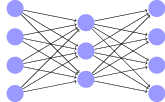
\includegraphics[width = 1.5cm]{figures/MLP.png} 
  } (tx.south);
  \node at (nn.south) {$q(x)$};
  \draw [->,dashed] (d.west) to[out = 180,in = 180] (z.west);
  \draw [->,dashed] (tx.west) -- (z.east);
  \end{tikzpicture}
  \caption{DSL $\mathcal{D}$ generates programs $p$ by sampling DSL primitives with probabilities $\theta$ (Algorithm~\ref{programGenerativeModel}). We observe program outputs $x$. A neural network $q(\cdot )$ called the \emph{recognition model} regresses from program outputs to a distribution over programs ($\theta^{(x)} = q(x)$). Solid arrows correspond to the top-down generative model. Dashed arrows correspond to the bottom-up recognition model.}\label{graphicalModel}
\end{figure}

\section{The \system Algorithm}

The goal of \system is to both induce a DSL and find good programs solving each of the tasks.
Our strategy is to iterate through three steps: (1) searching for programs that
solve the tasks, (2) learning a better neural recognition model -- which we use
to accelerate the search over programs -- and (3) improving the DSL.
The key observation here is that each of these three steps can bootstrap off of each other:

\begin{itemize}
  \item Searching for programs: Program search uses a distribution determined by the neural recognition model --
  so the recognition model bootstraps the search process.
  \item Learning a recognition model: The recognition model is trained both on samples from the DSL and on programs found by the search procedure. As the DSL improves and we find more programs, the recognition model gets both more data to train on and better data.
  \item Improving the DSL: We induce a DSL from the programs we have found so far which solve the tasks;
  as we solve more tasks, we can hone in on richer DSLs that more closely match the domain.
\end{itemize}

Section~\ref{mathematicalFraming} frames this 3-step procedure as
a means of maximizing a lower bound on the posterior probability of the DSL given the tasks.
Section~\ref{explorationSection} explains how we search for programs that solve the tasks;
Section~\ref{recognitionSection} explains how we train a neural network to accelerate the search over programs; and
Section~\ref{grammarInductionSection} explains how \system induces a DSL from programs.

\subsection{Probabilistic Framing}\label{mathematicalFraming}

\system takes as input a set of \emph{tasks}, written $X$, each of which is a program induction problem.
It has at its disposal a \emph{likelihood model}, written $\probability[x|p]$, which scores the likelihood of a task $x\in X$ given a program $p$.
Its goal is to solve each of the tasks by writing a program,
and also to infer a DSL $\mathcal{D}$ that distills the commonalities across all of the programs that solve the tasks.

We frame this problem as maximum a posteriori (MAP) inference in the generative model diagrammed in Fig.~\ref{graphicalModel}. We wish to maximize the MAP probability of $\mathcal{D}$:
\begin{equation*}
  \probability[\mathcal{D}|X]\propto \probability[\mathcal{D}] \int \mathrm{d}\theta P(\theta|\mathcal{D})\prod_{x\in X} \sum_p \probability[x|p]\probability[p|\mathcal{D},\theta]
\end{equation*}
In general this marginalization over $\theta$ is intractable, so we make an AIC-style approximation\footnote{Sec.~\ref{grammarInductionSection} explains that $\mathcal{D}$ is a context-sensitive grammar.
Conventional NLP approaches to using variational inference to lower bound the marginal over $\theta$ do not apply in our setting.}, $A\approx \log\probability[\mathcal{D}|X] $:
\begin{align}
  A =   \log \probability[\mathcal{D}] + \argmax_{\theta}& \sum_{x\in X}\log \sum_p\probability[x|p]\probability[p|\mathcal{D},\theta]\nonumber\\
&+  \log P(\theta|\mathcal{D}) - ||\theta||_0 \label{AIC}
  \end{align}


If we had a $(\mathcal{D},\theta)$ maximizing Eq.~\ref{AIC}, then we could recover the most likely program for task $x$ by maximizing $\probability[x|p] \probability[p|\mathcal{D},\theta]$.
Through this lens we now take as our goal to maximize Eq.~\ref{AIC}.
But even \emph{evaluating} Eq.~\ref{AIC} is intractable because it involves summing over the infinite set of all possible programs. In general, programs are hard-won: finding even a single program that explains a given observation presents a daunting combinatorial search problem.
With this fact in mind, we will instead maximize the following tractable lower bound on Eq.~\ref{AIC},
which we call $J$:
\begin{equation}
J = \log \probability[\mathcal{D},\theta] + \sum_{x\in X}\log \sum_{p\in \mathcal{F}_x} \probability[x|p]\probability[p|\mathcal{D},\theta]\label{lowerBound}
\end{equation}
This lower bound depends on sets of programs, $\left\{\mathcal{F}_x \right\}_{x\in X}$:

\noindent\textbf{Definition.} The \emph{frontier of task $x$}, written $\mathcal{F}_x$,
is a set of programs where $\probability[x|p] > 0$ for all $p\in \mathcal{F}_x$.

We maximize $J$ by alternatingly maximizing it w.r.t. the DSL and the frontiers:
%So interleaved with the DSL induction steps are program induction steps. Section~\ref{explorationSection}
%explains how \system synthesizes new programs and given a DSL.
\\\noindent \textbf{Program Search: Maxing $J$ w.r.t. the frontiers.} Here we
want to find new programs to add to  the frontiers so that $J$ increases the most.
Adding new programs to the frontiers means searching for new programs $p$ for task $x$
where $\probability[x,p|\mathcal{D},\theta]$ is large.
\\\noindent \textbf{DSL Induction: Maxing $J$ w.r.t. the DSL.} Here $\left\{\mathcal{F}_x \right\}_{x\in X}$ is held fixed and so we can evaluate $J$. Now the problem is that of searching the discrete space of DSLs and finding one maximizing $J$.

Searching for programs is extremely difficult because
of how large the search space is. We ease the difficulty of the search by learning a neural recognition model:

\textbf{Neural recognition model: tractably maxing $J$ w.r.t. the
  frontiers.}  Here we train a neural network, $q$, to predict a
distribution over programs conditioned on a task. The objective of $q$
is to assign high probability to programs $p$ where
$\probability[x,p|\mathcal{D},\theta]$ is large.  With $q$ in hand we can find programs for
frontier $\mathcal{F}_x$ by searching for programs maximizing
$q(p|x)$.
The network $q$ exploits the structure of the DSL $\mathcal{D}$:
rather than directly predicting a distribution over $p$ conditioned on $x$,
it predicts a weight vector, $\theta^{(x)}$, and we define $q(p|x)\triangleq \probability[p|\mathcal{D},\theta = q(x)]$.
This approach implements an amortized
inference scheme~\cite{ritchie2016deep} for the generative model in
Fig.~\ref{graphicalModel}.



%% Learning the DSL eases the difficulty of synthesis
%% by exposing a domain-specific basis for constructing programs.
%% Another complementary means of meeting search is to learn a
%% bottom-up \emph{recognition model}

\subsection{Searching for Programs}\label{explorationSection}

Now our goal is to search for programs that solve the tasks.  In this
work we use the simple search strategy of enumerating programs from
the DSL  in decreasing order of their probability,
and then checking if an enumerated program $p$ assigns positive
probability to a task ($\probability[x|p] > 0$); if so, we include $p$ in
the frontier $\mathcal{F}_x$.

To make this concrete we need to define what programs actually are and
what form $\probability[p |\mathcal{D},\theta]$ takes.
In this work, we represent programs as \emph{polymorphicly-type $\lambda$-calculus expressions}.
$\lambda$-calculus is a formalism for expressing functional programs.
It includes variables, function application, and the ability to create new functions using ...

TODO: summarize lambda calculus and types in one paragraph

\noindent\textbf{Definition: $\mathcal{D}$.}
A DSL $\mathcal{D}$ is a set of typed $\lambda$-calculus expressions.
\\\noindent\textbf{Definition: $\theta$.}
A weight vector $\theta$ for a DSL $\mathcal{D}$ is a vector of $|\mathcal{D}| + 1$ real numbers:
one number for each DSL primitive $e:\tau\in \mathcal{D}$, written $\theta_e$,
and a weight controlling the probability of a variable occurring in a program, written $\theta_{\text{var}}$.

Algorithm~\ref{programGenerativeModel} is a procedure for drawing
samples from $\probability[p|\mathcal{D},\theta]$.  In practice, we
enumerate programs rather than sampling them.  Enumeration proceeds by
a depth-first search over the random choices made by
Algorithm~\ref{programGenerativeModel}; we wrap the depth-first search
in iterative deepening to (approximately) build $\lambda$-calculus
expressions in order of their probability.



\begin{algorithm}[tb]
   \caption{Generative model over programs}
   \label{programGenerativeModel}
   \begin{algorithmic}
     \STATE \textbf{function} sampleProgramFromDSL$(\mathcal{D}, \theta, \tau)$:
  \STATE {\bfseries Input:} DSL $\mathcal{D}$, weight vector $\theta$, type $\tau$
  \STATE \textbf{Output:} a program whose type unifies with $\tau$
  \STATE \textbf{return} sample$(\mathcal{D}, \theta, \varnothing, \tau)$
\STATE
     \STATE \textbf{function} sample$(\mathcal{D}, \theta, \mathcal{E}, \tau)$:
  \STATE {\bfseries Input:} DSL $\mathcal{D}$, weight vector $\theta$, environment $\mathcal{E}$, type $\tau$
  \STATE \textbf{Output:} a program whose type unifies with $\tau$
  \IF{$\tau = \alpha\to\beta$}
  \STATE var $\gets$ an unused variable name
  \STATE body $\sim$ sample$(\mathcal{D},\theta,\{\text{var}:\alpha\}\cup\mathcal{E},\beta)$
   \STATE \textbf{return} $\lambda \text{var}.$ body
   \ENDIF
   %   \ELSE
   \STATE $\text{primitives} \gets\{p | &p: \tau' \in \mathcal{D}\cup\mathcal{E}$
   \STATE \hspace{2.5cm}$\text{if }\tau\text{ can unify with yield}(\tau')) \} $
   
   \STATE Draw $e\sim \text{primitives}$, w.p. $\propto\theta_e$ if $e\in \mathcal{D}$
   \STATE \hspace{3.1cm}w.p. $\propto\frac{\theta_{var}}{|\text{variables}|}$ if $e\in \mathcal{E}$
   \STATE Let $e:\alpha_1\to\alpha_2\to\cdots\to \alpha_K\to\beta$. Unify $\tau$ with $\beta$.
%   \STATE unify$(\tau,\beta)$
   \FOR{$k=1$ {\bfseries to} $K$}
 \STATE $a_k\sim\text{sample}(\mathcal{D},\theta,\mathcal{E},\alpha_k)$
 \ENDFOR
 \STATE \textbf{return} $e\;a_1\; a_2\; \cdots\; a_K$
 \STATE
 \STATE \textbf{function} yield$(\tau)$:
 \STATE \textbf{Input:} type $\tau$
 \STATE \textbf{Output:} the return type of $\tau$
 \STATE \textbf{if} $\tau = \alpha\to \beta$ \textbf{then return }yield$(\beta)$ \textbf{else return }$\tau$
\end{algorithmic}
\end{algorithm}

Why enumerate, when the program synthesis community has invented many
sophisticated algorithms that search for programs?~\cite{solar2008program,schkufza2013stochastic,feser2015synthesizing,osera2015type,polozov2015flashmeta}.
We have two reasons:% for using the simple strategy of enumerating programs:
\begin{itemize}
\item Enumeration is a general approach that can be applied to any program induction problem. Many of these more sophisticated approaches require special conditions on
  the space of of programs.
\item A key point of our work is that learning the DSL, along with a neural recognition model, can make program induction tractable, even if the
  search algorithm is very simple.  
\end{itemize}
A main drawback of an enumerative search algorithm is that we have no
efficient means of solving for arbitrary constants that might occur in the
program. In Section~\ref{regressionSection},
we will show how to find programs with real-valued constants
by automatically differentiating through the program and setting the constants using gradient descent.
In Section~\ref{textSection}
we will show that the bottom-up neural recognition model can learn
which discrete constants should be included in a program.







\subsection{Learning a Neural Recognition Model}\label{recognitionSection}

The purpose of the recognition model is to accelerate the search over
programs.  It does this by learning to predict which programs both 
assign high likelihood to a task, and at the same time 
have high prior probability under the prior $\probability[\cdot |\mathcal{D},\theta]$.

The recognition model $q$ is a neural network that predicts,
for each task $x\in X$, a weight vector $q(x) = \theta^{(x)}\in \mathbb{R}^{|\mathcal{D}| + 1}$.
Together with the DSL, this defines a distribution over programs,
$\probability[p|\mathcal{D},\theta = q(x)]$.
We abbreviate this distribution as $q(p|x)$.
The crucial aspect of this framing is that the neural network
can leverage the structure of the DSL,
and is \emph{not} responsible for
generating programs wholesale.
We will show that this lets us get away with a simple, low-capacity neural network.



We want a recognition model that closely approximates the true posteriors over programs, and so aim to minimize the following KL-divergence:
\begin{equation*}
  \expect\left[\text{KL}\left(\probability[p|x,\mathcal{D},\theta]||q(p|x) \right) \right]
\end{equation*}
which is equivalent to maximizing
$$
  \expect\left[\sum_p\probability[p|x,\mathcal{D},\theta]\log q(p|x) \right]
$$
  where the expectation is taken over tasks. One could take this expectation
  over the empirical distribution of the observations,
  like how an autoencoder is trained~\cite{hinton2006reducing}; or, one could take this expectation over samples from the generative model, like how a Helmholtz machine is trained~\cite{dayan1995helmholtz}.
  We found it useful to maximize both an autoencoder-style objective (written $\mathcal{L}_{\text{AE}}$) and a Helmholtz-style objective ($\mathcal{L}_{\text{HM}}$), giving the \system objective for a recognition model, $\mathcal{L}_{\text{RM}}$:
  \begin{align}
  \mathcal{L}_{\text{RM}}& = \mathcal{L}_\text{AE} + \mathcal{L}_\text{HM}\\
  \mathcal{L}_{\text{HM}}& = \expect_{p\sim(\mathcal{D},\theta) }\left[\log q(p|x)\right],\text{ $p$ evaluates to $x$}\nonumber\\
  \mathcal{L}_{\text{AE}}& = \expect_{x\sim X}\left[\sum_{p\in \mathcal{F}_x}
    \frac{\probability\left[x,p|\mathcal{D},\theta \right]}{\sum_{p'\in \mathcal{F}_x}\probability\left[x,p|\mathcal{D},\theta \right]}\log q(p|x)\right]\nonumber
  \end{align}

  Evaluating $\mathcal{L}_{\text{HM}}$ involves sampling programs from
  the current DSL, running them to get their outputs,
  and then training $q$ to regress from the outputs to the program.
  If these programs map inputs to outputs,
  then we need some way of sampling these inputs as well.
  Our solution to this problem is to sample the inputs
  from the empirical observed distribution of inputs in $X$.

\subsection{Inducing the DSL from the Frontiers}\label{grammarInductionSection}

The purpose of the DSL is to
offer a set of abstractions
that allow an agent to easily express solutions to the tasks at hand.
In the \system algorithm we infer the DSL from a collection of frontiers.
Intuitively, we want the algorithm to
look at the programs in the frontiers and
generalize beyond them; 
not only so the DSL can better express the current solutions,
but also so that the DSL might expose new abstractions
which will later used to
discover even better programs.

Exact maximization of $J$ (Eq.\ref{lowerBound}) w.r.t. $(\mathcal{D},\theta)$
is intractable,
so we take a more heuristic approach.
The strategy is to search locally through the space of DSLs,
proposing small local changes to $\mathcal{D}$ until $J$ fails to increase.
The search moves work by introducing new
$\lambda$-expressions into the DSL.
We propose these new expressions by extracting subexpressions from
programs already in the frontier.
These extracted subexpressions
are fragments of the original programs, and can introduce new variables (Figure~\ref{fragmentExample}),
which then become new functions in the DSL.

Closely related to Fragment Grammars~\cite{tim} and Tree-Substitution Grammars~\cite{cohn2010inducing},
but context-sensitive

We define a prior distribution over DSLs which penalizes the sizes of the $\lambda$-calculus expressions in the DSL, and put a Dirichlet prior over the weight vector:
\begin{align*}
  \probability[\mathcal{D}]&\propto\exp\left(\lambda\sum_{p\in \mathcal{D}}\text{size}(p) \right)\\
  P(\theta|\mathcal{D})& = \text{Dir}(\theta|\alpha)
\end{align*}
where $\text{size}(p)$  measures the size of the syntax tree of program $p$,
$\lambda$ is a hyperparameter that acts as a regularizer on the size of the DSL,
and $\alpha$ is a concentration parameter controlling the smoothness of the prior over $\theta$.
Algorithm~\ref{grammarInductionAlgorithm} specifies the DSL induction algorithm.

Additionally, for each proposed $\mathcal{D}$ we have to reestimate $\theta$.
Although this problem may seem 
very similar to estimating the parameters of a probabilistic context free grammar (PCFG: see~\cite{}),
for which we have effective approaches like the Inside/Outside algorithm~\cite{international2000derivation},
$\mathcal{D}$
 is actually context-sensitive
due to the presence of variables in the programs and also due to the
polymorphic typing system.
In the Appendix we derive an efficient MAP estimator for $\theta$.

\begin{algorithm}[tb]
   \caption{DSL Induction Algorithm}
   \label{grammarInductionAlgorithm}
   \begin{algorithmic}
     \STATE {\bfseries Input:} Set of frontiers $\{\mathcal{F}_x\}$
     \STATE \textbf{Hyperparameters:} Pseudocounts $\alpha$, regularization parameter $\lambda$
     \STATE \textbf{Output:} DSL $\mathcal{D}$, weight vector $\theta$
     \STATE Define $L(\mathcal{D},\theta) =  \prod_x \sum_{z\in \mathcal{F}_x} \probability[z|\mathcal{D},\theta]$
     \STATE Define $\theta^*(\mathcal{D}) = \argmax_\theta \text{Dir}(\theta|\alpha) L(\mathcal{D},\theta)$
     \STATE Define $\text{score}(\mathcal{D}) = \log \probability[\mathcal{D}] + L(\mathcal{D},\theta^*) - ||\theta||_0$
     \STATE $\mathcal{D}\gets$ every primitive in $\{\mathcal{F}_x\}$
     \WHILE {true}
     \STATE N $\gets \{\mathcal{D}\cup \{s\} | x\in X, z\in \mathcal{F}_x, s\text{ subexpression of }z\}$
     \STATE $\mathcal{D}'\gets \argmax_{\mathcal{D}'\in N}\text{score}(\mathcal{D}') $
     \STATE \textbf{if }$\text{score}(\mathcal{D}') < \text{score}(\mathcal{D})$\textbf{ return }$\mathcal{D},\theta^*(\mathcal{D})$
     \STATE $\mathcal{D}\gets\mathcal{D}'$
     \ENDWHILE
   \end{algorithmic}
\end{algorithm}

\begin{figure*}
  \begin{tabular}{lll}
    \toprule
    Domain&Example programs in frontiers&Example proposed subexpression\\\midrule
    Boolean circuits&
    \begin{tabular}{l}
      \texttt{(lambda x (nand x x))}\\
      \texttt{(lambda x (lambda y (nand x (nand y y))}
    \end{tabular}&
    \texttt{(nand z z)}\\\midrule
    String editing&
    \begin{tabular}{l}
      \texttt{(lambda s (+ ',' (index 0 (split ',' s))))}\\
      \texttt{(lambda s (index 0 (split ' ' s)))}
    \end{tabular}&
    \texttt{(index 0 (split z s))}\\\bottomrule
  \end{tabular}
  \caption{The DSL induction algorithm works by proposing subexpressions of programs to add to the DSL.
    These subexpressions are taken from programs in the frontiers (middle column), and can introduce new variables (\texttt{z} in the right column).}
  \label{fragmentExample}
  \end{figure*}


\section{Experiments}

\subsection{Boolean circuits}
pedagogical example; easy domain
\begin{figure}
  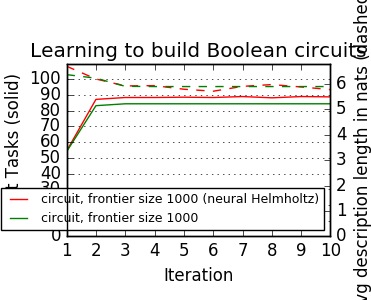
\includegraphics[width = \columnwidth]{figures/circuit.png} 
\end{figure}

\subsection{Symbolic Regression}\label{regressionSection}
We show how to use \system to infer programs containing both discrete
structure and continuous parameters. The high-level idea is to synthesize programs with unspecified-real-valued parameters, and to fit those parameters using gradient descent.
Concretely, we ask the algorithm to
solve a set of 1000 symbolic regression problems, each a polynomial of
degree 0, 1, or 2, where our observations $x$ take the form of $N$
input/output examples, which we write as $x = \left\{(i_n,o_n)
\right\}_{n\leq N}$. For example, one task is to infer a program
calculating $3x + 2$, and the observations are the input-output
examples $\left\{(-1,-1),(0,2),(1,5) \right\}$.

We initially equip our DSL learner with addition and multiplication,
along with the possibility of introducing real-valued parameters, which we write as $\mathcal{R}$.
We define the likelihood of an observation $x$ by assuming a Gaussian noise model for the input/output examples and integrate over the real-valued parameters, which we collectively write as $\vec{\mathcal{R}}$:
\begin{align*}
\log   \probability\left[\{(i_n,o_n)\}|p\right] = \log \int \mathrm{d}\vec{\mathcal{R}}\; P_{\vec{\mathcal{R}}}(\vec{\mathcal{R}})\prod_{n\leq N}\mathcal{N}(p(i_n,\vec{\mathcal{R}})|o_n)
%\text{\emph{BIC:}} &\approx 
\end{align*}
where $\mathcal{N}(\cdot |\cdot )$ is the normal density  and $P_{\vec{\mathcal{R}}}(\cdot )$ is a prior over $\vec{\mathcal{R}}$. We approximate this marginal using the BIC~\cite{Bishop:2006:PRM:1162264}:
\begin{align*}
  \log \probability[x|p]  \approx& \sum_{n\leq N}\log \mathcal{N}(p(i_n,\vec{\mathcal{R}}^*)|o_n) - \frac{D\log N}{2}
\end{align*}
where $\vec{\mathcal{R}}^*$ is an assignment to $\vec{\mathcal{R}}$ found by performing gradient ascent on the likelihood of the observations w.r.t. $\vec{\mathcal{R}}$.

What DSL does \system learn?
The learned DSL contains templates for quadratic and linear functions,
which lets the algorithm quickly hone in on the kinds of functions that are most appropriate to this domain.
Examining the programs themselves,
one finds that the algorithm discovers representations for each of the polynomials that minimizes the number of continuous degrees of freedom:
for example, it represents the polynomial $8x^2+8x$

\begin{tabular}{ll}
  \toprule
  Primitives& $+,\times:\mathbb{R}\to \mathbb{R}\to \mathbb{R}$\\
  & $\mathcal{R}:\mathbb{R}$ (real valued parameter)\\\midrule
  Observation $x$& $N$ input/output examples: $\left\{(i_n,o_n) \right\}_{n\leq N}$\\
  \midrule
  Likelihood $\probability[x|p]$& $\propto\exp\left( - D\log N \right)\prod_{n\leq N}\mathcal{N}(p(i_n)|o_n)$
  \\\midrule
  \begin{tabular}{l}
    Subset of \\Learned DSL
    \end{tabular}&
  \begin{tabular}{ll}
    $\lambda x. \mathcal{R}\times x + \mathcal{R}$ &linear\\
    $\lambda x. \mathcal{R} + x$ &increment\\
    $\lambda x. x\times (\text{linear } x)$&$\text{quadratic}_0$\\
    $\lambda x. \text{increment }(\text{quadratic}_0\; x)$&quadratic\\
  \end{tabular}
  \\\bottomrule
  \end{tabular}

\begin{figure}
      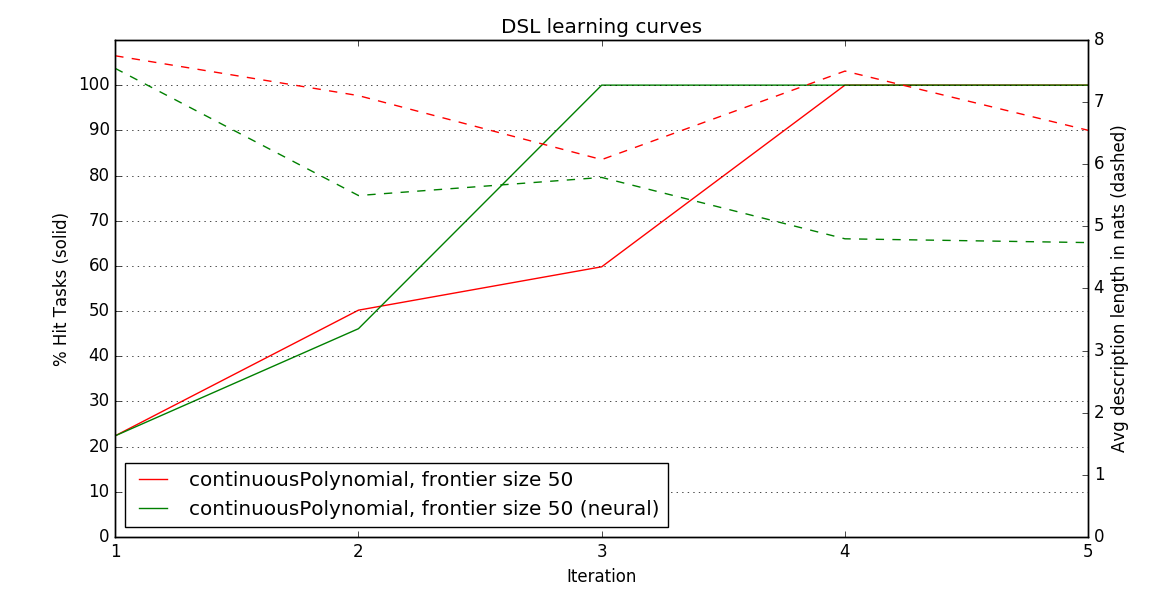
\includegraphics[width = 9cm]{figures/polynomial.png}
\end{figure}
\subsection{String editing}\label{textSection}
\begin{figure}

  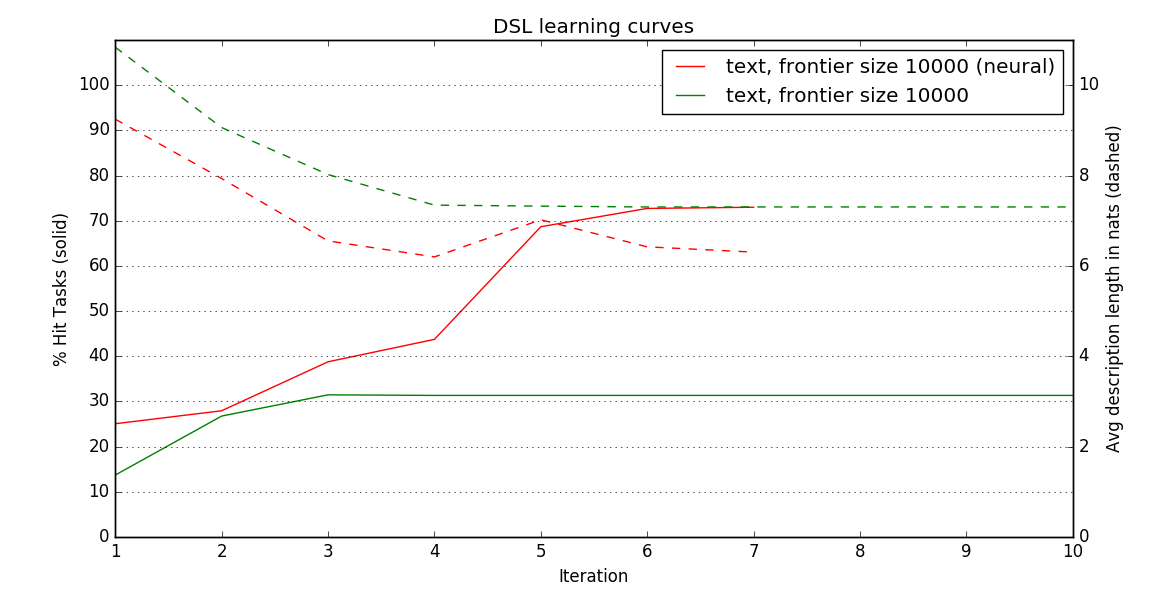
\includegraphics[width = 9cm]{figures/text.png}

\end{figure}

\subsection{List functions}
Our list function domain consists of tasks which are solved by functions
that take as input an integer or a list of integers, and have as output
either a Boolean, an integer, or a list of integers. Examples of these
functions are in Table~\ref{listexamples}. For each function, we create a
task $x$ by generating 15 input/output examples used for testing whether a
program produces the correct output. Supplying many examples reduces
ambiguity in the task's function, ensuring solutions achieve the desired
concept.

\begin{table}
\centering
\begin{tabular}{| l | l | l |}
  \hline
  \emph{name} & \emph{input} & \emph{output} \\
  \hline
  add-3 & [1\, 2\, 3\, 4] & [4\, 5\, 6\, 7] \\
  append-4 & [7\, 0\, 2] & [7\, 0\, 2\, 4] \\
  len & [3\, 5\, 12\, 1] & 4 \\
  range & 3 & [1\, 2\, 3] \\
  has-2 & [4\, 5\, 7\, 4] & \texttt{false} \\
  has-4 & [4\, 5\, 7\, 4] & \texttt{true} \\
  repeat-2 & [7\, 0] & [7\, 0\, 7\, 0] \\
  drop-3 & [0\, 3\, 8\, 6\, 4] & [6\, 4] \\
  \hline
\end{tabular}
\caption{Examples from the domain of list functions.}
\label{listexamples}
\end{table}

We supply \system with the DSL outlined in Table~\ref{listdsl}.

\begin{table}
\centering
\begin{tabular}{| l | l |}
  \hline
  \emph{name} & \emph{type} \\
  \hline
    empty & \texttt{tlist($\alpha$)} \\
    singleton & \texttt{arrow($\alpha$, tlist($\alpha$))} \\
    range & \texttt{int $\rightarrow$ tlist(int)} \\
    concat & \texttt{tlist($\alpha$) $\rightarrow$ tlist($\alpha$) $\rightarrow$ tlist($\alpha$)} \\
    map & \texttt{($\alpha$ $\rightarrow$ $\beta$) $\rightarrow$ tlist($\alpha$) $\rightarrow$ tlist($\beta$)} \\
    reduce & \texttt{($\beta$ $\rightarrow$ $\alpha$ $\rightarrow$ $\beta$) $\rightarrow$ $\beta$ $\rightarrow$ tlist($\alpha$) $\rightarrow$ $\beta$} \\
    \hline
    true & \texttt{bool} \\
    not & \texttt{bool $\rightarrow$ bool} \\
    and & \texttt{bool $\rightarrow$ bool $\rightarrow$ bool} \\
    or & \texttt{bool $\rightarrow$ bool $\rightarrow$ bool} \\
    \hline
    0, $\ldots$, 9 & \texttt{int} \\
    + & \texttt{int $\rightarrow$ int $\rightarrow$ int} \\
    * & \texttt{int $\rightarrow$ int $\rightarrow$ int} \\
    negate & \texttt{int $\rightarrow$ int} \\
    mod & \texttt{int $\rightarrow$ int $\rightarrow$ int} \\
    eq? & \texttt{int $\rightarrow$ int $\rightarrow$ bool} \\
    gt? & \texttt{int $\rightarrow$ int $\rightarrow$ bool} \\
    is-prime & \texttt{int $\rightarrow$ bool} \\
    is-square & \texttt{int $\rightarrow$ bool} \\
    sort & \texttt{tlist(int) $\rightarrow$ tlist(int)} \\
    \hline
    sum & \texttt{tlist(int) $\rightarrow$ int} \\
    reverse & \texttt{tlist($\alpha$) $\rightarrow$ tlist($\alpha$)} \\
    all & \texttt{($\alpha$ $\rightarrow$ bool) $\rightarrow$ tlist($\alpha$) $\rightarrow$ bool} \\
    any & \texttt{($\alpha$ $\rightarrow$ bool) $\rightarrow$ tlist($\alpha$) $\rightarrow$ bool} \\
    index & \texttt{int $\rightarrow$ tlist($\alpha$) $\rightarrow$ $\alpha$} \\
    filter & \texttt{($\alpha$ $\rightarrow$ bool) $\rightarrow$ tlist($\alpha$) $\rightarrow$ tlist($\alpha$)} \\
    slice & \texttt{int $\rightarrow$ int $\rightarrow$ tlist($\alpha$) $\rightarrow$ tlist($\alpha$)} \\
  \hline
\end{tabular}
\caption{DSL for the domain of list function.}
\label{listdsl}
\end{table}

\begin{figure}
  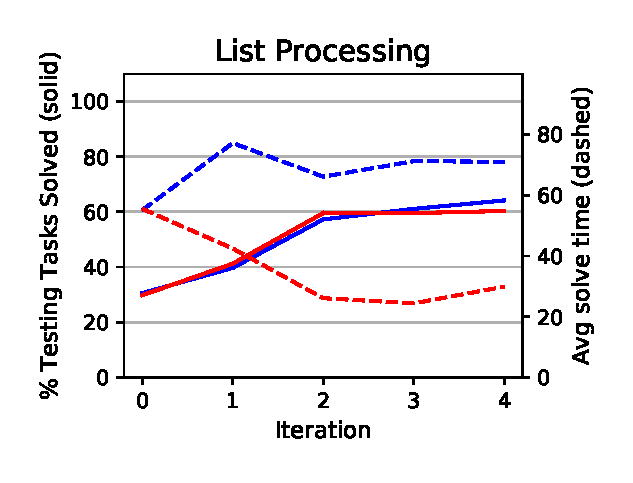
\includegraphics[width=\columnwidth]{figures/list.eps}
\end{figure}

We found that using a less sophisticated but equally-capable DSL made common
patterns, such as summation, unlikely and unlearnable in a small enumeration
bound.

\section{Model}







\begin{algorithm}[tb]
   \caption{DSL Learner}
   \label{mainAlgorithm}
   \begin{algorithmic}
     \STATE {\bfseries Input:} Initial DSL $\mathcal{D}$, set of tasks $X$, iterations $I$
     \STATE \textbf{Hyperparameters:} Frontier size $F$
     \STATE \textbf{Output:} DSL $\mathcal{D}$, weight vector $\theta$, bottom-up recognition model $q(\cdot)$
     \STATE Initialize $\mathcal{D}_0\gets \mathcal{D}$, $\theta_0\gets \text{uniform}$, $q_0(\cdot ) = \theta_0$
     \FOR{$i=1$ {\bfseries to} $I$}
     \FOR{$x:\tau\in X$}
     \STATE  $\mathcal{F}_x\gets \{z| z\in \text{enumerate}(\mathcal{D}_{i - 1},q_{i - 1}(x),F)\cup\text{enumerate}(\mathcal{D}_{i - 1},\theta_{i - 1},F) \text{ if }\probability[x|z] > 0\}$
     \ENDFOR
     \STATE $\mathcal{D}_i,\theta_i\gets $induceGrammar$(\{\mathcal{F}_x\}_{x\in X})$
     \STATE Define $Q_x(z) \propto \begin{cases}
       \probability[x|z]\probability[z|\mathcal{D}_i,\theta_i]&x\in \mathcal{F}_x\\
       0&x\not \in \mathcal{F}_x
     \end{cases}$
     \STATE $q_i\gets \argmin_q \sum_{x\in X}\text{KL}(Q_x(\cdot )||\probability[\cdot |\mathcal{D}_i,q(x)])$
      \ENDFOR
 \STATE \textbf{return} $\mathcal{D}^I,\theta^I,q^I$
\end{algorithmic}
\end{algorithm}

\pagebreak

\section{Program Representation}
We choose to represent programs using $\lambda$-calculus~\cite{pierce}.
A $\lambda$-calculus expression is either:
\\\noindent A \emph{primitive}, like the number 5 or
  the function \texttt{sum}.
\\\noindent A \emph{variable}, like $x$, $y$, $z$
\\\noindent A $\lambda$\emph{-abstraction}, which creates a new function. $\lambda$-abstractions have a variable and a body. The body is a $\lambda$-calculus expression. Abstractions are written as $\lambda \text{var}. \text{body}$.
\\\noindent An \emph{application} of a function to an argument. Both the function and the argument are $\lambda$-calculus expressions. The application of the function $f$ to the argument $x$ is written as $f\; x$.

For example, the function which squares the logarithm of a number is
$\lambda x.\text{\texttt{square}} (\text{\texttt{log} } x)$, and the identity function $f(x) = x$ is $\lambda x.x$. The
$\lambda$-calculus serves as a spartan but expressive Turing complete
program representation, and distills the essential features of functional languages like Lisp.

However, many $\lambda$-calculus expressions correspond to ill-typed programs, such as the program that takes the logarithm of the Boolean \texttt{true} (i.e., \texttt{log true}) or which applies the number five to the identity function
(i.e., $5 \; (\lambda x.x)$).
We use a well-established typing system for $\lambda$-calculus called \emph{Hindley-Milner typing}~\cite{pierce}, which is used in programming languages like OCaml.
The purpose of the typing system is to ensure that our programs never call a function with a type it is not expecting (like trying to take the logarithm of \texttt{true}).
Hindley-Milner has two important features:
Feature 1: It supports \emph{parametric polymorphism}: meaning that types can have variables in them, called \emph{type variables}. Lowercase Greek letters are conventionally used for  type variables.
For example, the type of the identity function is $\alpha\to\alpha$, meaning it takes something of type $\alpha$ and return something of type $\alpha$. A function that returns the first element of a list has the type $\texttt{list}(\alpha)\to\alpha$. Type variables are not the same has variables introduced by $\lambda$-abstractions.
Feature 2: Remarkably, there is a  simple algorithm for automatically inferring the polymorphic Hindley-Milner type of a $\lambda$-calculus expression~\cite{damas1982principal}.
A detailed exposition of Hindley-Milner is beyond the scope of this work.

%% \begin{figure}
%%   \begin{align}
%%     \text{primitive types} & 
%%     \end{align}
%%   \end{figure}



\section{Estimating $\theta$}



We write $c(e,p)$ to mean the number of times that primitive $e$ was used in program $p$;  $R(p)$ to mean the sequence of types input to sample in Alg.\ref{programGenerativeModel}. Jensen's inequality gives an intuitive lower bound on the likelihood of a program $p$:
\begin{align*}
  \log \probability[p|\theta]&\stackrel{+}{ = }\sum_{e\in \mathcal{D}} c(e,p)\log \theta_e - \sum_{\tau\in R(p)} \log \sum_{\substack{e:\tau'\in \mathcal{D}\\\text{unify}(\tau,\tau')}}\theta_e\\
  &\stackrel{+}{\geq }\sum_{e\in \mathcal{D}} c(e,p)\log \theta_e - c(p)\log \sum_{\tau\in R(p)} \sum_{\substack{e:\tau'\in \mathcal{D}\\\text{unify}(\tau,\tau')}}\theta_e\\
  & = \sum_{e\in \mathcal{D}} c(e,p)\log \theta_e - c(p)\log \sum_{e\in \mathcal{D}} r(e,p)\theta_e
\end{align}
where $c(p) = \sum_{e\in \mathcal{D}}c(e,p)$ and $r(e:\tau',p) = \sum_{\tau\in R(p)} \indicator[\text{canUnify}(\tau,\tau')]$.

Differentiate with respect to $\theta_e$ and set to zero 
\begin{align}
  \frac{c(x)}{\theta^{(x)}} &= N\frac{a(x)}{\sum_y a(y)\theta_y}
\end{align}
This equality holds if $\theta^{(x)} = c(x)/a(x)$:
\begin{align}
  \frac{c(x)}{\theta_x} &= a(x).\\
N\frac{a(x)}{\sum_y a(y)\theta_y}& = N\frac{a(x)}{\sum_y c(y)}   = N\frac{a(x)}{N} = a(x).
\end{align}
If this equality holds then $\theta_x \propto c(x)/a(x)$:
\begin{align}
  \theta_x = \frac{c(x)}{a(x)}\times \underbrace{\frac{\sum_y a(y)\theta_y}{N}}_{\text{Independent of $x$}}.
\end{align}

Now what we are actually after is the parameters that maximize the joint log probability of the data+parameters, which I will write $J$:
\begin{align}
  J& = L + \log \text{D}(\theta|\alpha)\\
  &\stackrel{+}{\geq } \sum_x c(x)\log \theta_x - N \log \sum_x a(x)\theta_x  + \sum_x(\alpha_x - 1)\log \theta_x\\
  & = \sum_x (c(x) + \alpha_x - 1)\log \theta_x -  N \log \sum_x a(x)\theta_x
\end{align}
So you add the pseudocounts to the \emph{counts} ($c(x)$), but not to the \emph{possible counts} ($a(x)$).


\bibliography{main}
\bibliographystyle{icml2018}

\end{document}


% This document was modified from the file originally made available by
% Pat Langley and Andrea Danyluk for ICML-2K. This version was created
% by Iain Murray in 2018. It was modified from a version from Dan Roy in
% 2017, which was based on a version from Lise Getoor and Tobias
% Scheffer, which was slightly modified from the 2010 version by
% Thorsten Joachims & Johannes Fuernkranz, slightly modified from the
% 2009 version by Kiri Wagstaff and Sam Roweis's 2008 version, which is
% slightly modified from Prasad Tadepalli's 2007 version which is a
% lightly changed version of the previous year's version by Andrew
% Moore, which was in turn edited from those of Kristian Kersting and
% Codrina Lauth. Alex Smola contributed to the algorithmic style files.
